\section{Calculated Inputs}
\label{sec:usingStatisticalInput}
As described in the Section~\ref{sec:annSection} and in Figure~\ref{fig:overfitting} the Neural Network strives for a generalized function without over-fitting so that it also applies for data outside of the trained set. In order to achieve such a function it is necessary to include enough input parameters to get a close enough fit. Every input parameter should narrow down the possible number of output values or else it makes no sense to include them. What can become problematic is when the input parameters simply result in too many output values, e.g. if similar wind speeds, air densities and temperatures would correspond to wind productions between 800-1300 \todo{concrete example from data set}. The generalization would move towards the majority of the wind productions in the interval but because the purpose of prediction is to come as close as possible to the ideal value this is not enough when the interval is too big. One way to solve this is to include a "snapshot" of the current situation and add it as input to the network so that it takes into account market trends at that time. The purpose is to add additional characteristics of the time-series that are currently used for training. As discussed in Historical Data~\ref{sec:historicalData} the market has certain trends and if the prediction knows the production or price from one hour ago and the current market trend in general, it will possibly have a better chance of guessing within the given interval. If putting this into context of the wind production interval 800-1300; the last hour wind production being 1100 and a rising current trend should with high probability not guess around 800 even if the majority of the wind productions is placed here. The concept is illustrated in Figure~\ref{fig:WP}\todo{make drawing}. Including the current trend as input can help the ANN to better approach the target to predict because it  would calculate how current trend in general influences the output over the entire dataset. The trend input parameter would be a probability for the curve to either go up or down at every step. This can potentially cause problematic situations when facing steep rising or falling slopes, provided that such exist, because the ANN would not predict high or low enough since the trend says nothing about the slope but only if the trend is rising or falling. A possible solution could be to include inputs telling something about the current slope. One such input could be a simple curve analysis where the slope of the last prices or productions are taken into consideration as well. The slope says something about how much the curve in general is rising whereas the statistics will reflect the general trend, are we moving up or down, over time. If the majority of the slopes in the dataset is falling the network would predict according to that. If we are facing a steep slope we won't be able to predict high enough since the slope is out of the ordinary. Events could be related to socio-cultural events that are beyond the scope of this thesis like the financial crisis or the breakdown of power plants.

Other problems arise together with the inclusion of tendency --- when have we moved enough in one direction? We need to rely on the other input parameters to pull us either up or down so that we can identify the next trend. The dataset used for training must be big enough to reflect most trends or else problems can occur when meeting new trends in the unseen data for prediction, e.g. if most trends in general are rising in the training set and then trying to predict 24 hours that are not would result in a disproportion between the two sets. The possibility of over-shooting the first targets would be high since it has never seen such trends before.    It will need to be tested thoroughly during our experiments. 

One thing to keep in mind here is that the trend and slope are only a minority of the input parameters. Without these the Artificial Neural Network would have made one generalization and the assumptions is that it will help the function to approach the target better when a lot of output possibilities exist. The result will be a new function where the immediate past is considered at every hour and the possibility of a improved generalization.

\begin{figure}[H]
\centering
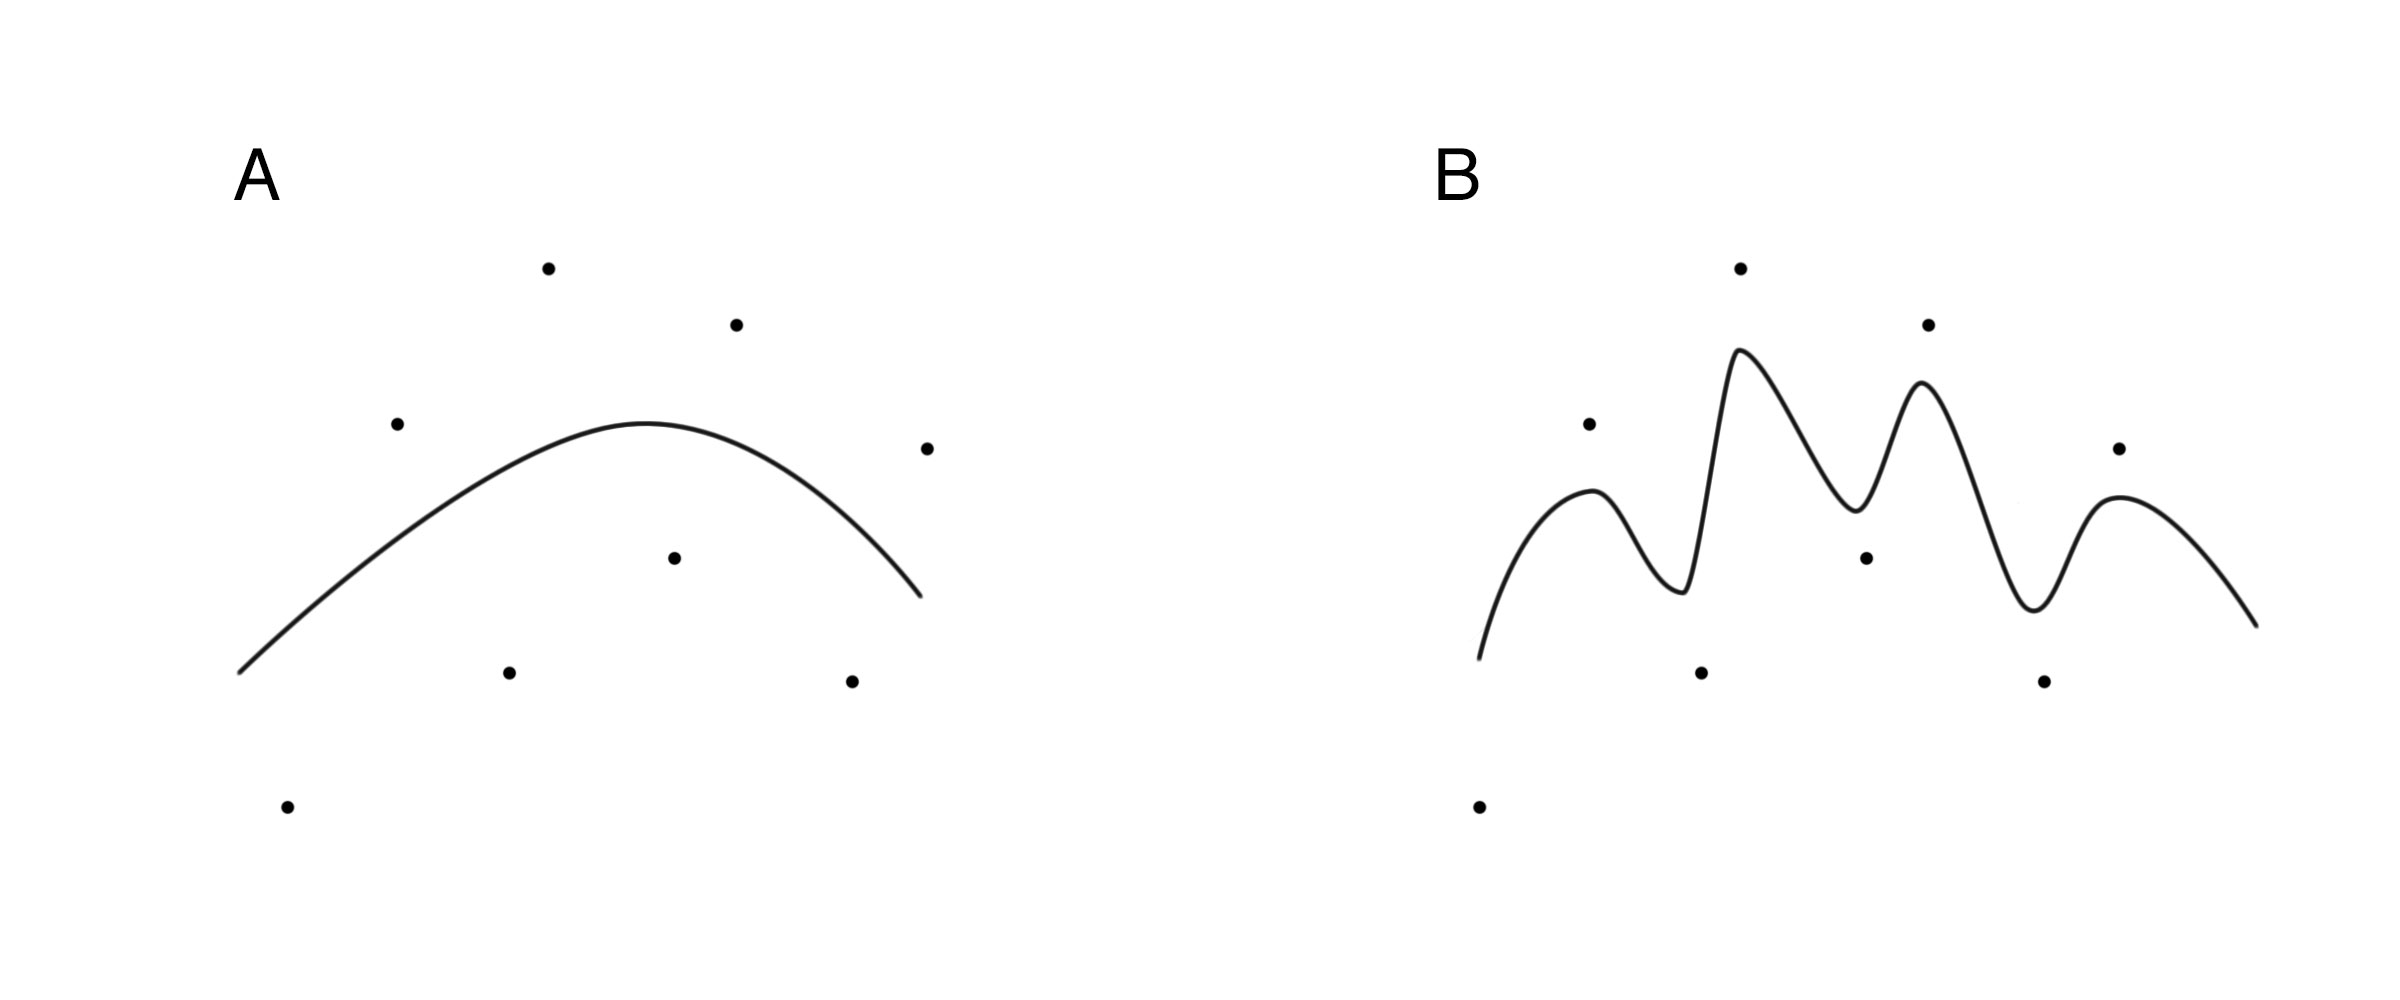
\includegraphics[width=0.99\linewidth,natwidth=898,natheight=587]{billeder/WP_000057.jpg}
\caption{A) Shows the generalized function. B) The approaching of output values}
\label{fig:WP}
\end{figure}

We will work with several statistical methods as input and with combinations of them all. 

\subsection{Curve Analysis}
\label{sec:curveAnalysis}

\subsection{Scatter}

\subsection{EWMA - Historical Volatility}
\label{sec:ewmaVolatility}
\todo{Talk about statistical input features like historical volatility (EWMA), skewness and basic calculation of line slope. Skewness is a more sophisticated way of calculating if the distribution is leaning to one sine of the mean - the simple line slope calculation is meant to calculate if we are on the way up or down}

EWMA should be used for time series that do not have a clear trend direction\cite[Chapter~7.3.2]{econometrics} which is exactly what we have. \todo{see page 588 in econometrics book}. EWMA is a latent trend model where a latent variable is included to describe a discrete choice model. The latent variable is called the smoothing factor and if this factor is close to one then the last trend has a higher weight than the recent observation and when it is close to zero the new has higher priority and thereby letting the EWMA follow trends more rapidly - in our case the observation would be either production or price and the smoothing factor is calculated based on the last calculated trend. Choice of smoothing factor must be tested in experiments but since there is high volatility in both price and wind power production a lower factor could be expected. Every hour must calculate the historical volatility based on a defined number of previous hours. The exact number will also be found in experiments.

\subsection{Skewness}
\label{sec:skewness}




TEGNING MULTIPE STEP

TALK ABOUT MULTIPLE-STEP-AHEAD FORECASTING --> see karlbranting
